\documentclass{exam}

\usepackage{units} 
\usepackage[fleqn]{amsmath}
\usepackage{float}
\usepackage{mdwlist}
\usepackage{booktabs}
\usepackage{caption}
\usepackage{fullpage}
\usepackage{enumerate}
\usepackage{graphicx}

\usepackage{2in1, lscape} 
\setcounter{tocdepth}{1}
\everymath{\displaystyle}

\author{}
\date{January 22, 2014}
\title{Statistics \\ Week One}

\begin{document}

  \maketitle
  \tableofcontents

  \section{Death Penalty Case Study}
  
  \subsection{Data}
  \begin{table}[ht]
  \centering
  \begin{tabular}{rlllr}
    \toprule
          & defendant & victim & sentence  & count \\
    \midrule
    1     & white & white & death     & 19 \\
    2     & white & black & death     & 0 \\
    3     & white & white & not death & 112 \\
    4     & white & black & not death & 9 \\
    5     & black & white & death     & 11 \\
    6     & black & black & death     & 6 \\
    7     & black & white & not death & 52 \\
    8     & black & black & not death & 97 \\
    \midrule
    total &       &       &           & 306 \\
    \bottomrule
  \end{tabular}
  \end{table}

  \subsection{By Sentence}

  12\% of the death penalty eligible cases with convictions resulted in death penalties.

  \begin{table}[H]
    \centering
    \begin{tabular}{rlrrr}
      \toprule
      & Cases & DP & Percent \\
      \midrule
      & 306   & 36 & 12 \\
     \bottomrule
    \end{tabular}
    \caption{All Cases}
  \end{table}

  \subsection{By Defendant Race}

  White defendants are more likely to get the death penalty than black defendants.

  \begin{table}[H]
    \centering
    \begin{tabular}{rlrrr}
      \toprule
        & Defendant & Cases & DP & Percent \\
      \midrule
      1 & black     & 166   & 17 & 10 \\
      2 & white     & 140   & 19 & 14 \\
      \bottomrule
    \end{tabular}
    \caption{By defendant race}
  \end{table}

  \subsection{By Defendant and Victim Race}

  For any race of victim, black defendants are more likely to get the death penalty than white defendants.

  \begin{table}[H]
    \centering
    \begin{tabular}{rllrrr}
      \hline
          & Defendant & Victim & Cases & DP & Percent \\
       1  & black     & black  & 103   & 6  & 6 \\
       2  & black     & white  & 63    & 11 & 17 \\
       3  & white     & black  & 9     & 0  & 0 \\
       4  & white     & white  & 131   & 19 & 15 \\
       \hline
    \end{tabular}
    \caption{By defendant and victim race}
  \end{table}

  \subsection{By Victim Race}

  Cases with white victims are much more likely to result in the death penalty than cases with black victims.
  \begin{table}[H]
    \centering
    \begin{tabular}{rlrrr}
      \toprule
        & Victim & Cases & DP & Percent \\
      \midrule
      1 & black  & 112   & 6  & 5 \\
      2 & white  & 194   & 30 & 15 \\
      \bottomrule
    \end{tabular}
  \end{table}

  \begin{figure}[H]
    \centering
    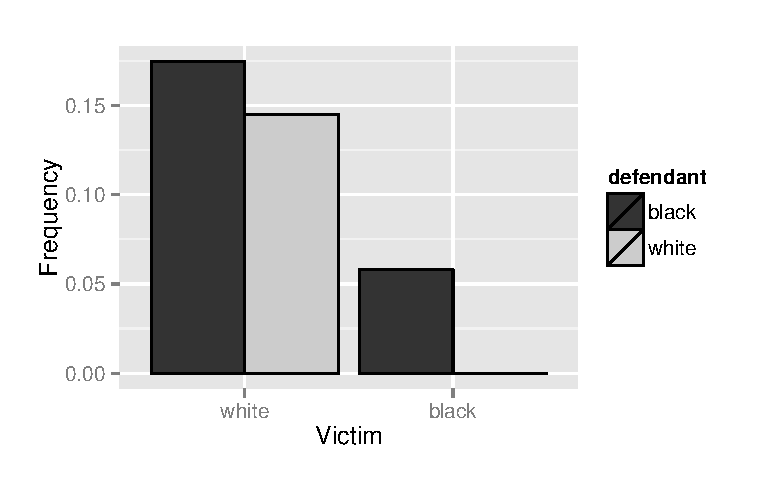
\includegraphics[scale = 0.9]{figures/death_penalty.eps}
    \caption{Death Penalty Summary}
  \end{figure}

  \section{Data Sets}
  \begin{itemize*}
    \item {\em Observation} is one row
    \item Columns are {\em variables}
    \item Quantitative variables are numbers that can take on any value like money, weight, number of people, etc.
    \item Category variables are things like male/female, state, car model, etc.
  \end{itemize*}

  \begin{table}[H]
    \centering
    \begin{tabular}{lrrrl}
      \toprule
      State       & Year & Population & Prison & region    \\
      \midrule
      Alabama     & 2010   & 4779736  & 26321  & South     \\
      Alaska      & 2010   & 710231   & 3771   & West      \\
      Arizona     & 2010   & 6392017  & 34774  & West      \\
      Arkansas    & 2010   & 2915918  & 14192  & South     \\
      California  & 2010   & 37253956 & 160651 & West      \\
      Colorado    & 2010   & 5029196  & 18254  & West      \\
      Connecticut & 2010   & 3574097  & 17746  & Northeast \\
      Delaware    & 2010   & 897934   & 6378   & South     \\
      Florida     & 2010   & 18801310 & 90274  & South     \\
      Georgia     & 2010   & 9687653  & 47561  & South     \\
      Hawaii      & 2010   & 1360301  & 3363   & West      \\
      Idaho       & 2010   & 1567582  & 4999   & West      \\
      \vdots      \\
      % Illinois       & 2010 & 12830632   & 48418  & Midwest   \\
      % Indiana        & 2010 & 6483802    & 24456  & Midwest   \\
      % Iowa           & 2010 & 3046355    & 9457   & Midwest   \\
      % Kansas         & 2010 & 2853118    & 9055   & Midwest   \\
      % Kentucky       & 2010 & 4339367    & 12374  & South     \\
      % Louisiana      & 2010 & 4533372    & 16087  & South     \\
      % Maine          & 2010 & 1328361    & 1954   & Northeast \\
      % Maryland       & 2010 & 5773552    & 22786  & South     \\
      % Massachusetts  & 2010 & 6547629    & 11162  & Northeast \\
      % Michigan       & 2010 & 9883640    & 44113  & Midwest   \\
      % Minnesota      & 2010 & 5303925    & 9397   & Midwest   \\
      % Mississippi    & 2010 & 2967297    & 11213  & South     \\
      % Missouri       & 2010 & 5988927    & 30577  & Midwest   \\
      % Montana        & 2010 & 989415     & 1635   & West      \\
      % Nebraska       & 2010 & 1826341    & 4608   & Midwest   \\
      % Nevada         & 2010 & 2700551    & 12192  & West      \\
      % New Hampshire  & 2010 & 1316470    & 2617   & Northeast \\
      % New Jersey     & 2010 & 8791894    & 21647  & Northeast \\
      % New Mexico     & 2010 & 2059179    & 3754   & West      \\
      % New York       & 2010 & 19378102   & 56420  & Northeast \\
      % North Carolina & 2010 & 9535483    & 40167  & South     \\
      % North Dakota   & 2010 & 672591     & 1416   & Midwest   \\
      % Ohio           & 2010 & 11536504   & 48671  & Midwest   \\
      % Oklahoma       & 2010 & 3751351    & 18128  & South     \\
      % Oregon         & 2010 & 3831074    & 13859  & West      \\
      % Pennsylvania   & 2010 & 12702379   & 47072  & Northeast \\
      % Rhode Island   & 2010 & 1052567    & 3159   & Northeast \\
      % South Carolina & 2010 & 4625364    & 22992  & South     \\
      % South Dakota   & 2010 & 814180     & 3388   & Midwest   \\
      % Tennessee      & 2010 & 6346105    & 14917  & South     \\
      % Texas          & 2010 & 25145561   & 141087 & South     \\
      % Utah           & 2010 & 2763885    & 5442   & West      \\
      % Vermont        & 2010 & 625741     & 1517   & Northeast \\
      % Virginia       & 2010 & 8001024    & 30351  & South     \\
      % Washington     & 2010 & 6724540    & 17028  & West      \\
      % West Virginia  & 2010 & 1852994    & 5072   & South     \\
      % Wisconsin      & 2010 & 5686986    & 21983  & Midwest   \\
      % Wyoming        & 2010 & 563626     & 1875   & West      \\
      \bottomrule
    \end{tabular}
    % \caption{Population and prison population for 2010}
  \end{table}

  \section{Time Graphs}

  \subsection{Overview}

  Time graphs show how a continuous variable changes over time.  

  \begin{itemize*}
    \item x-axis is time
    \item y-axis is the quantity being measured
    \item can use line or bar
  \end{itemize*}

  \subsection{US}
  \begin{figure}[H]
    \centering
    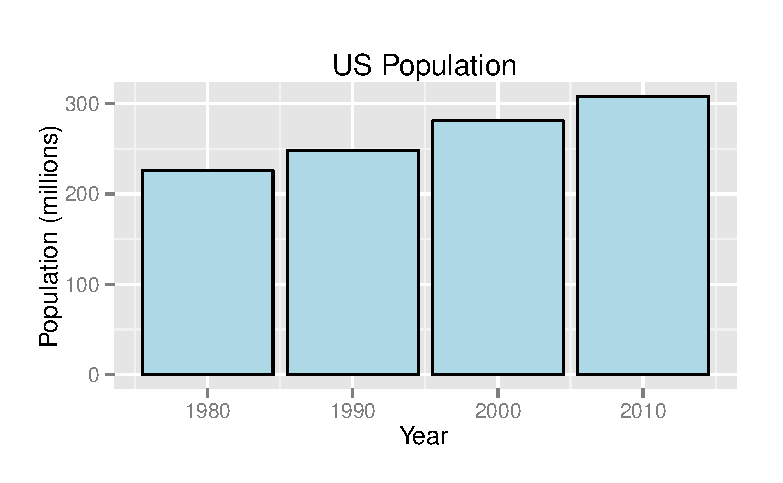
\includegraphics[scale = 0.9]{figures/us_population.eps}
    \caption{US population 1980 to 2010}
  \end{figure}

  You can make the growth rate look larger by changing the y-axis.
  \begin{figure}[H]
    \centering
    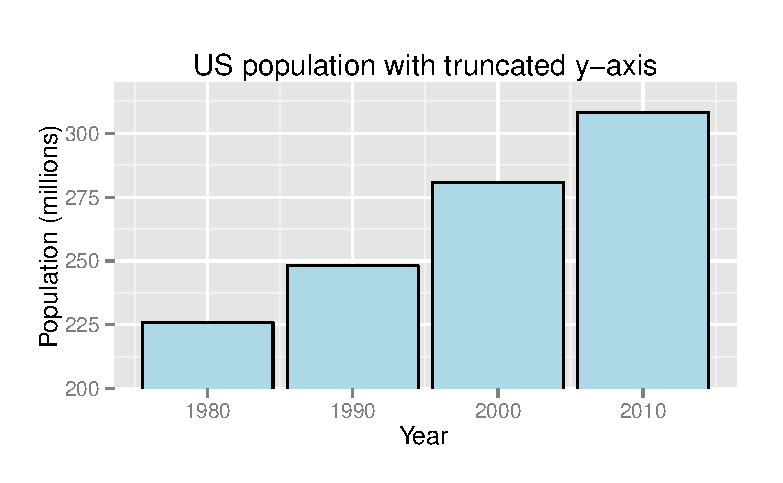
\includegraphics[scale = 0.9]{figures/us_population_limited_range.eps}
    \caption{US population with y-axis starting at 200}
  \end{figure}

  \begin{figure}[H]
    \centering
    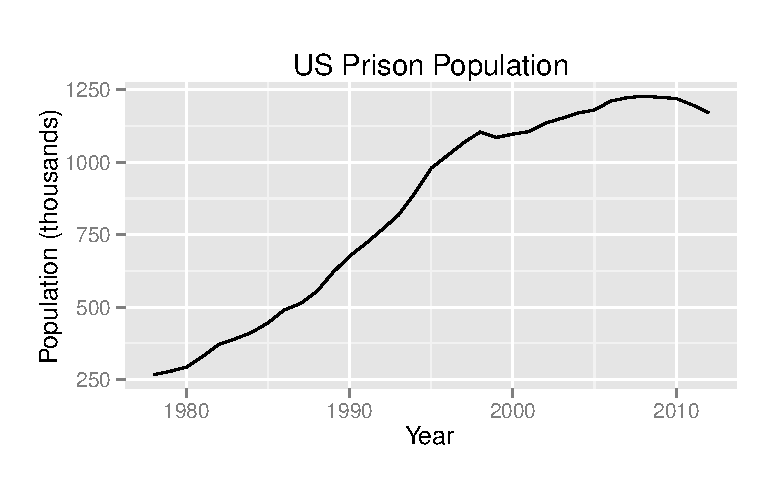
\includegraphics[scale = 0.9]{figures/us_prison_population.eps}
    \caption{US prison population}
  \end{figure}

  \begin{figure}[H]
    \centering
    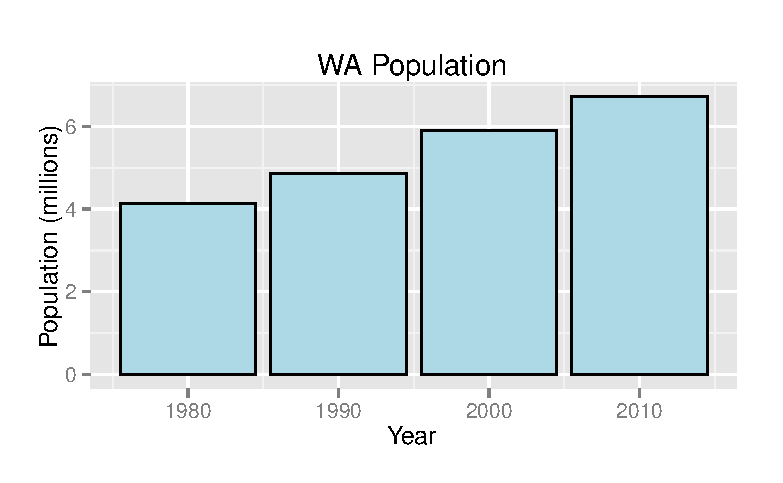
\includegraphics[scale = 0.9]{figures/wa_population.eps}
    \caption{WA population 1980-2010}
  \end{figure}

  \begin{figure}[H]
    \centering
    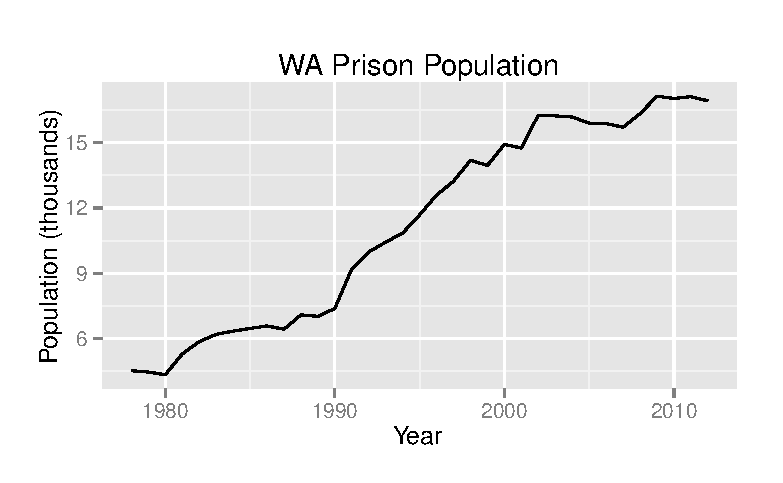
\includegraphics[scale = 0.9]{figures/wa_prison_population.eps}
    \caption{WA prison population 1980-2010}
  \end{figure}

  Talk about how the prison population goes up because of:
  \begin{itemize*}
    \item longer sentances
    \item making more crimes result in prison
    \item increased population
  \end{itemize*}

  \section{Bar Graphs}

  \subsection{Overview}
  \begin{itemize*}
    \item shows value for some quantitative variable for each value of a categorical variable
    \item x-axis is categorical variable (state, region, car model, color, etc.)
    \item y-axis is quantitative variable
  \end{itemize*}

  \subsection{States}

  \begin{figure}[H]
    \centering
    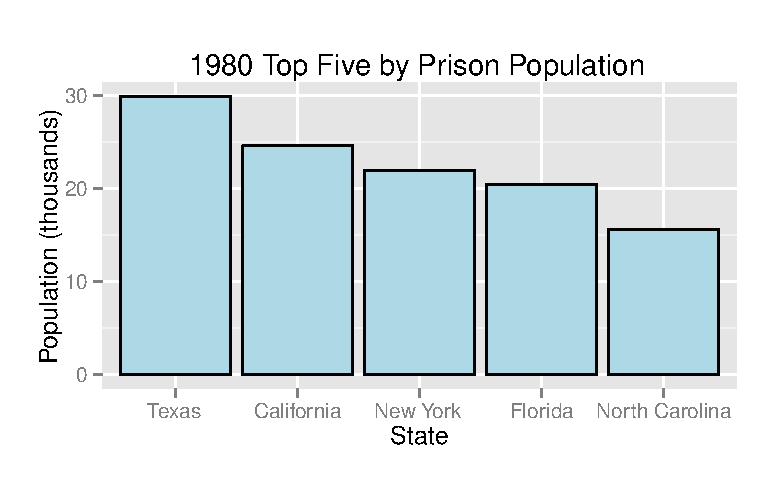
\includegraphics[scale = 0.9]{figures/top_five_1980.eps}
    \caption{1980 top five states by prison population}
  \end{figure}

  \begin{figure}[H]
    \centering
    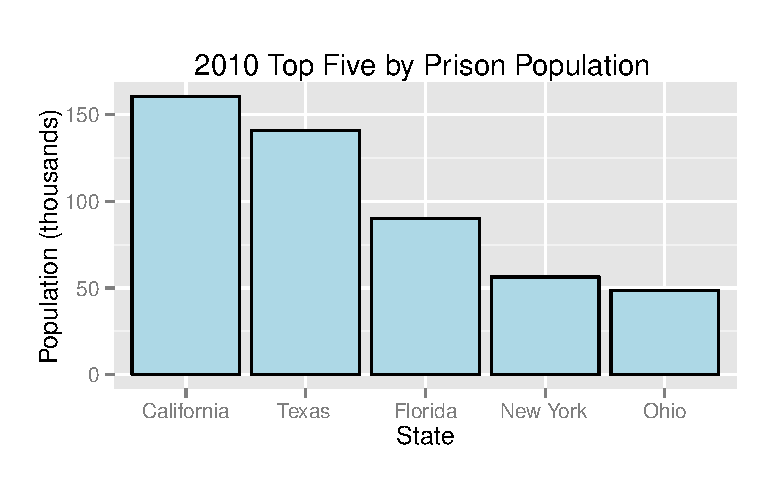
\includegraphics[scale = 0.9]{figures/top_five_2010.eps}
    \caption{2010 top five states by prison population}
  \end{figure}

  You can use the color to add a second categorical variable.
  \begin{figure}[H]
    \centering
    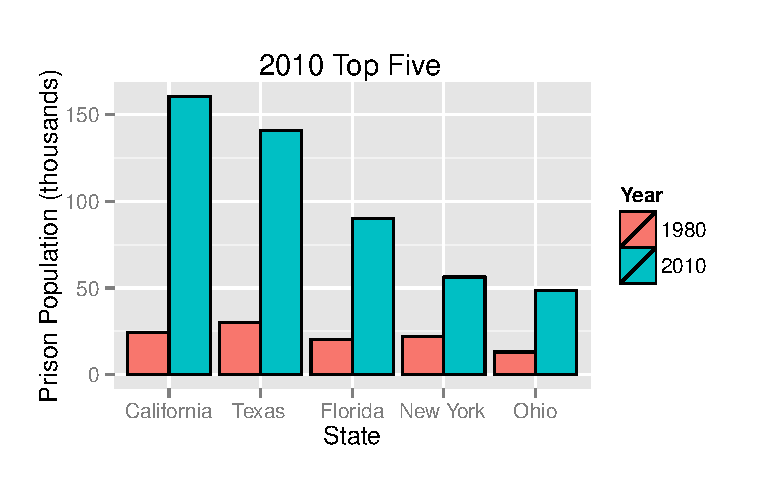
\includegraphics[scale = 0.9]{figures/1980_to_2010_top_five.eps}
    \caption{2010 vs. 1980 top five states by prison population}
  \end{figure}

  \subsection{Regions}
  \begin{figure}[H]
    \centering
    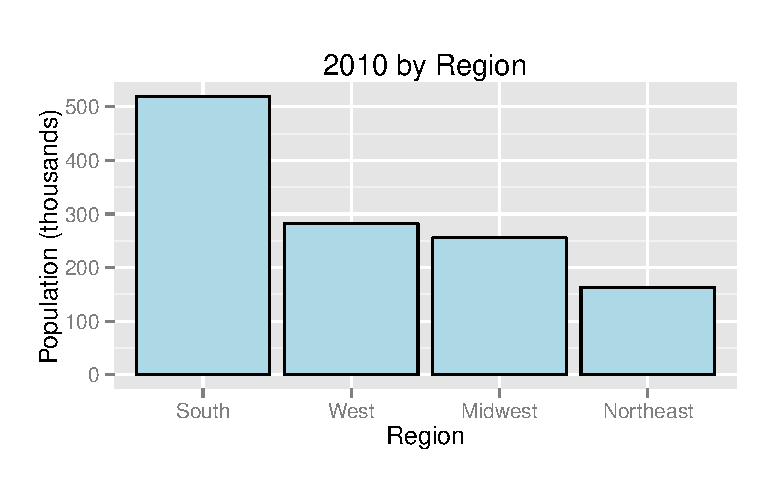
\includegraphics[scale = 0.9]{figures/regions_2010.eps}
    \caption{2010 by region}
  \end{figure}

  \begin{figure}[H]
    \centering
    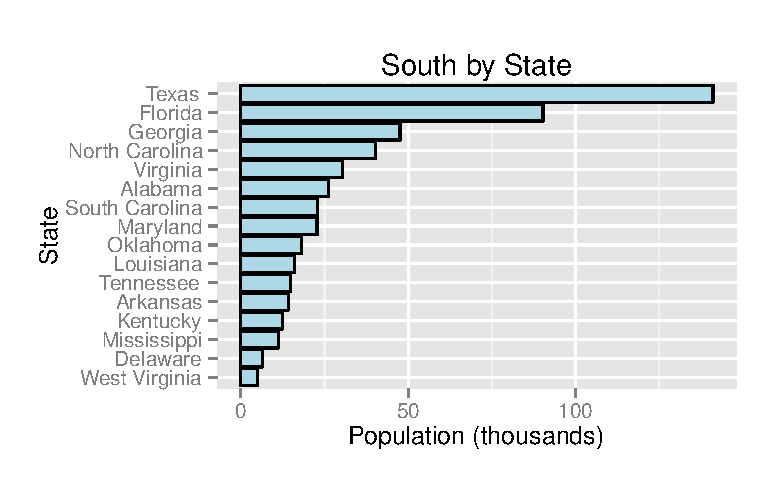
\includegraphics[scale = 0.9]{figures/south_by_state.eps}
    \caption{2010 southern region by state}
  \end{figure}

  \begin{figure}[H]
    \centering
    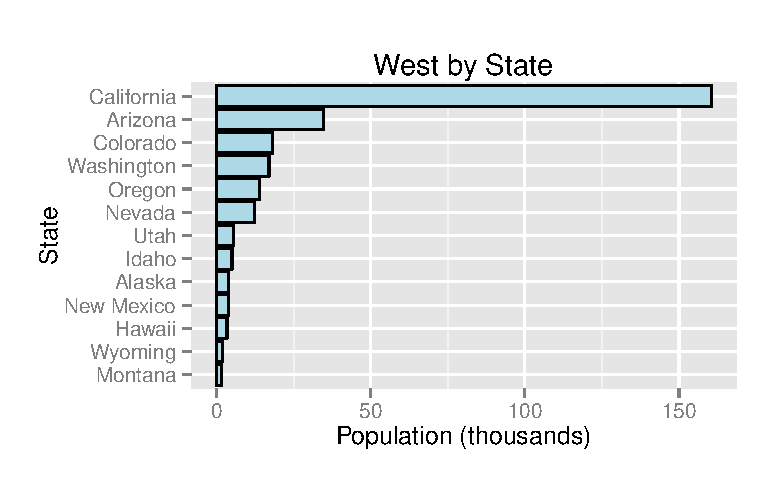
\includegraphics[scale = 0.9]{figures/west_by_state.eps}
    \caption{2010 western region by state}
  \end{figure}

  \begin{figure}[H]
    \centering
    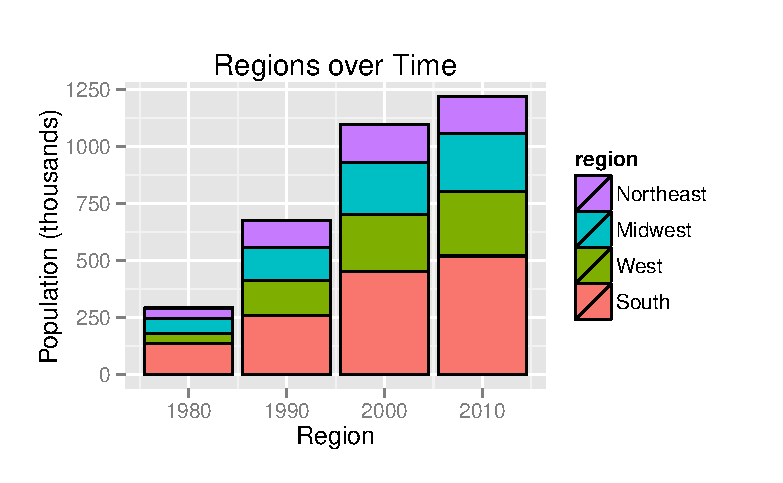
\includegraphics[scale = 0.9]{figures/regions_over_time.eps}
    \caption{Regional change over time}
  \end{figure}

  \begin{figure}[H]
    \centering
    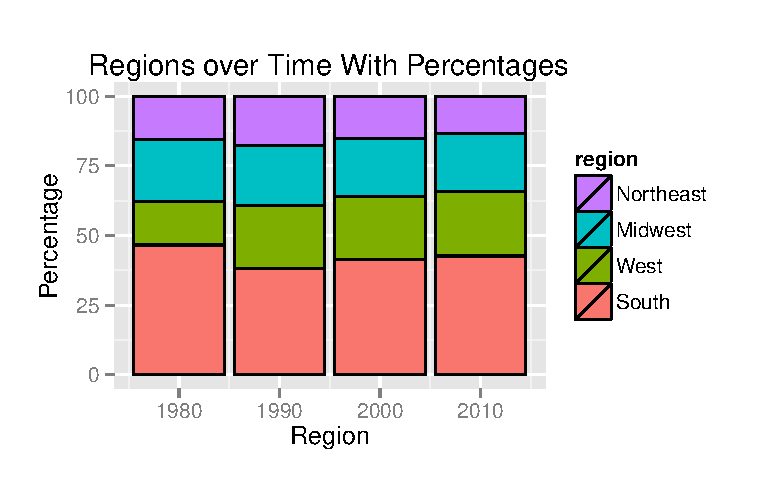
\includegraphics[scale = 0.9]{figures/regions_over_time_percentages.eps}
    \caption{Regional change over time with percentages}
  \end{figure}

  \section{Histograms}

  \subsection{Overview}
  \begin{itemize*}
    \item shows number of occurrences of quantitative variable by range
    \item x-axis is quantitative variable ranges
    \item y-axis is number of occurrences in each range
  \end{itemize*}

  \subsection{Stem Plots}
  \begin{itemize*}
    \item Describe how to make Stem Plots
    \item Use 2010 population data with stems of 10,000
    \item Describe how to split stems (0-4, 5-9, 10-14, 15-20, etc.).  With
      2010 data, this would give bin width of 5,000
  \end{itemize*}

  \subsection{Prison Population}

  \begin{figure}[H]
    \centering
    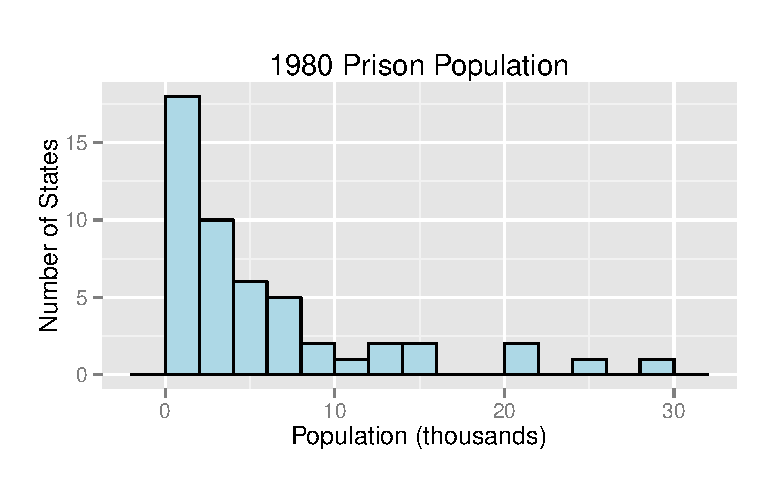
\includegraphics[scale = 0.9]{figures/population_histogram_1980.eps}
    \caption{1980 histogram}
  \end{figure}

  \begin{figure}[H]
    \centering
    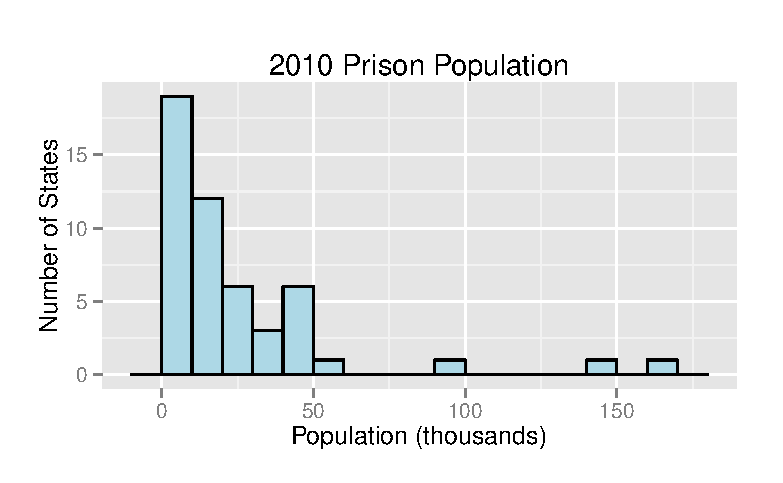
\includegraphics[scale = 0.9]{figures/population_histogram_2010.eps}
    \caption{2010 histogram}
  \end{figure}

  \begin{figure}[H]
    \centering
    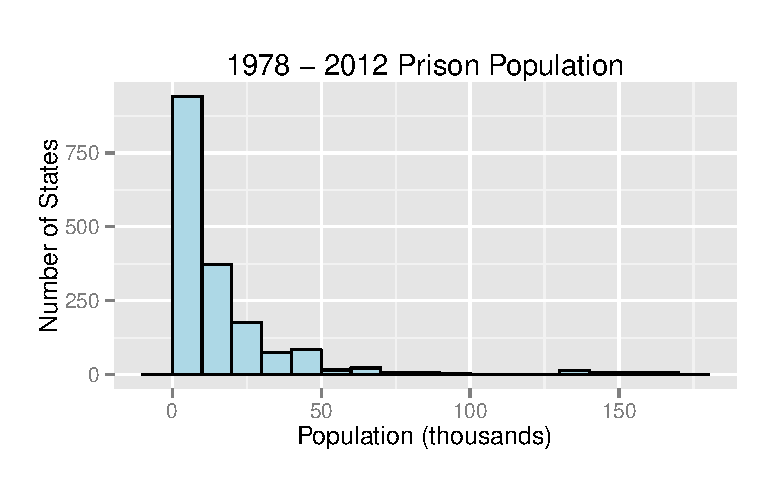
\includegraphics[scale = 0.9]{figures/population_histogram_all_years.eps}
    \caption{Histogram for all years (isn't very useful)}
  \end{figure}

  \begin{figure}[H]
    \centering
    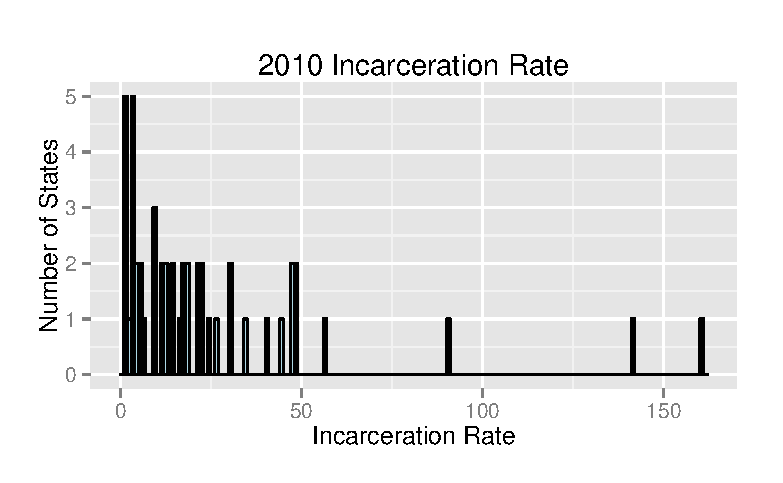
\includegraphics[scale = 0.9]{figures/population_histogram_2010_small_bins.eps}
    \caption{Histogram with too small bin size}
  \end{figure}

  \section{US Incarceration Rates}

  \subsection{1980}

  \begin{itemize*}
    \item median 104
    \item mean 121
    \item highest rate was 265 (North Carolina)
    \item lowest rate was 34 (New Hampshire)
    \item highest population was 29,892 (Texas)
    \item lowest population was 313 (New Hampshire)
    \item skewed right
  \end{itemize*}

  \begin{figure}[H]
    \centering
    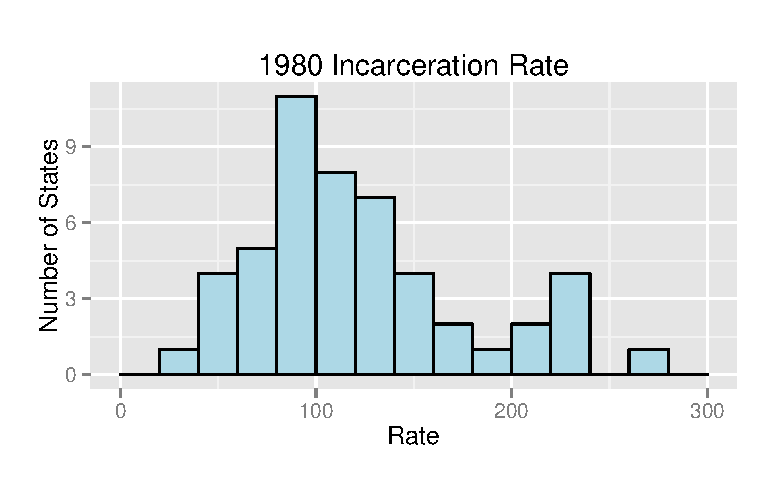
\includegraphics[scale = 0.9]{figures/rate_histogram_1980.eps}
  \end{figure}

  \begin{figure}[H]
    \centering
    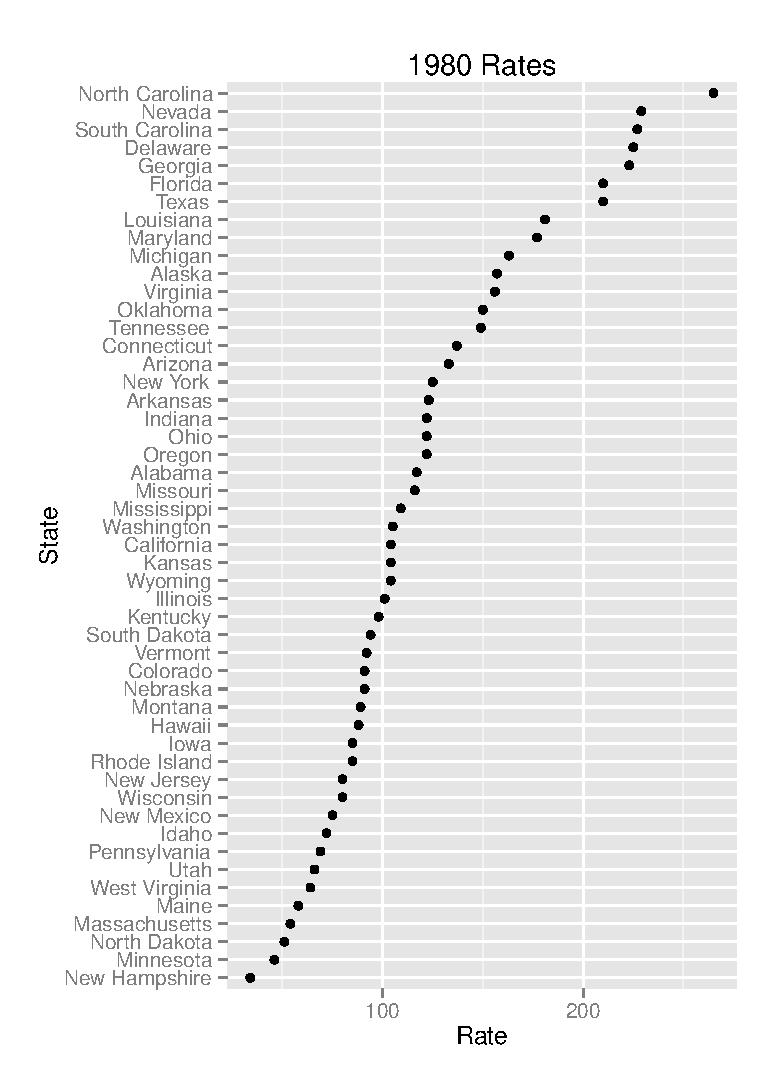
\includegraphics[scale = 0.9]{figures/state_rates_1980.eps}
    \caption{1980 rates}
  \end{figure}

  \subsection{2010}
  \begin{itemize*}
    \item median rate 367
    \item mean rate 360
    \item highest rate was 710 (Delaware)
    \item lowest rate was 147 (Maine)
    \item highest population was 160,651 (California)
    \item lowest population was 1,416 (North Dakota)
    \item Delaware is outlier
    \item symmetric
  \end{itemize*}

  \begin{figure}[H]
    \centering
    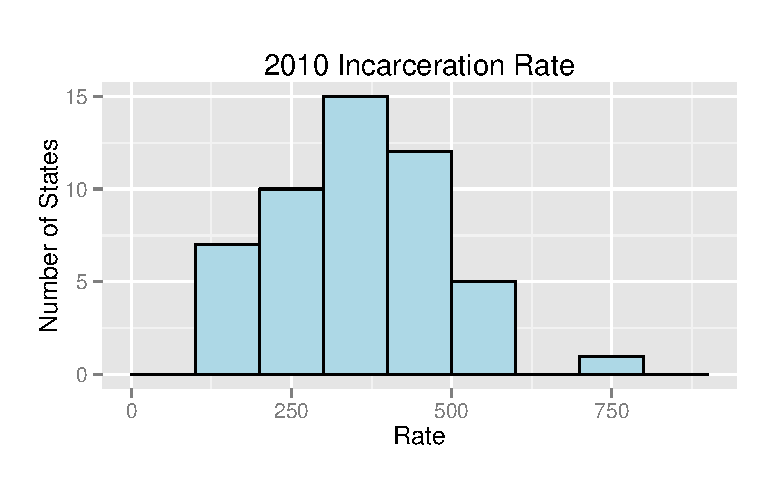
\includegraphics[scale = 0.9]{figures/rate_histogram_2010.eps}
  \end{figure}

  \begin{figure}[H]
    \centering
    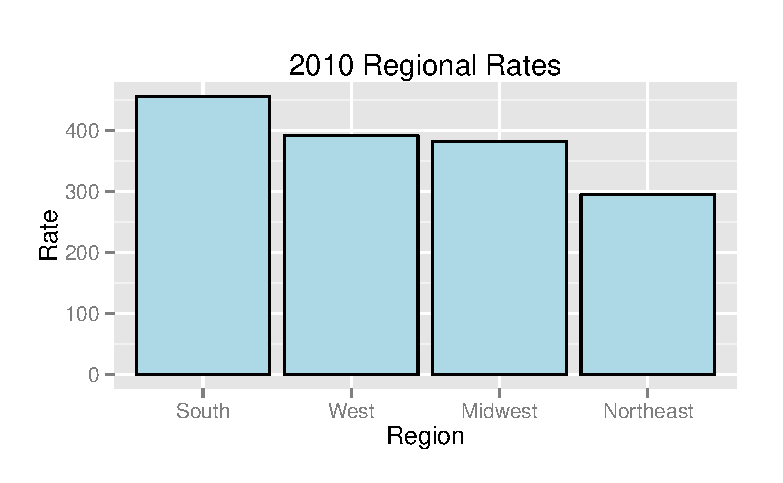
\includegraphics[scale = 0.9]{figures/regional_rates_2010.eps}
    \caption{2010 US regional rate.  Explain how regional rate is calculated.}
  \end{figure}

  \begin{figure}[H]
    \centering
    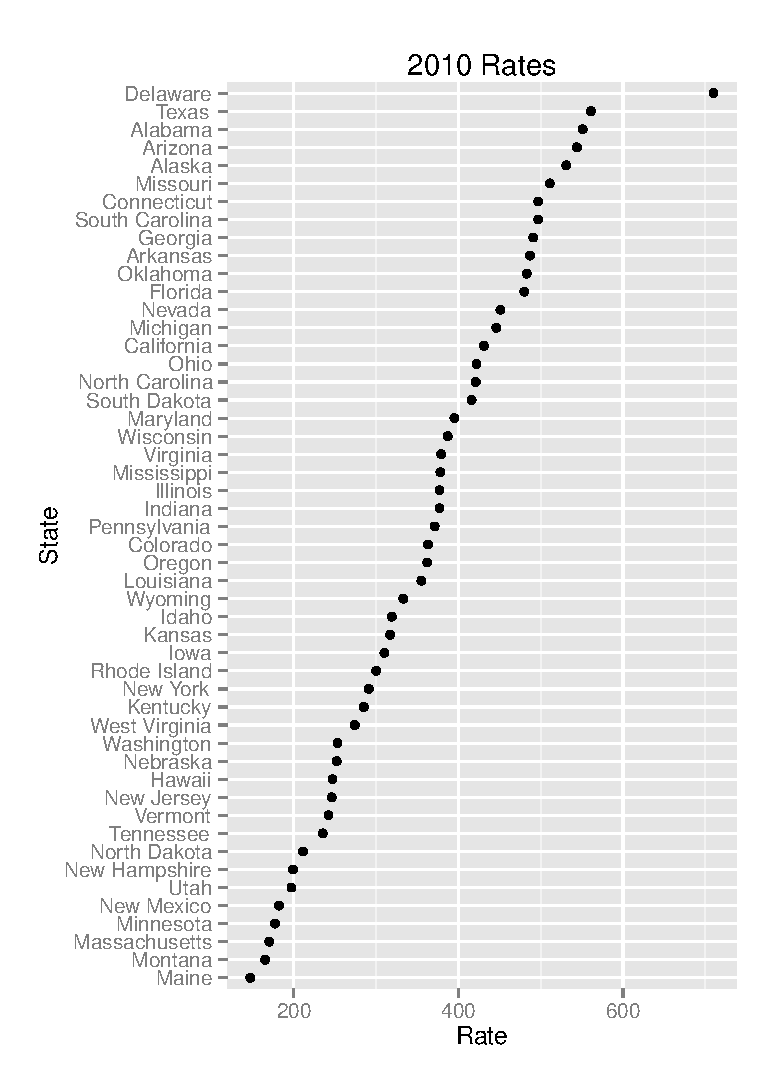
\includegraphics[scale = 0.9]{figures/state_rates_2010.eps}
    \caption{2010 rates}
  \end{figure}

  \subsection{Rates Over Time}
  \begin{figure}[H]
    \centering
    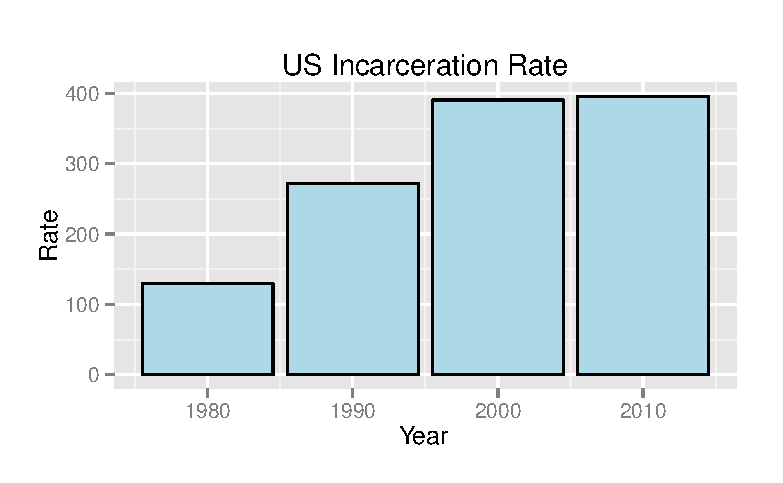
\includegraphics[scale = 0.9]{figures/us_rate_over_time.eps}
    \caption{US rate over time}
  \end{figure}

  \begin{figure}[H]
    \centering
    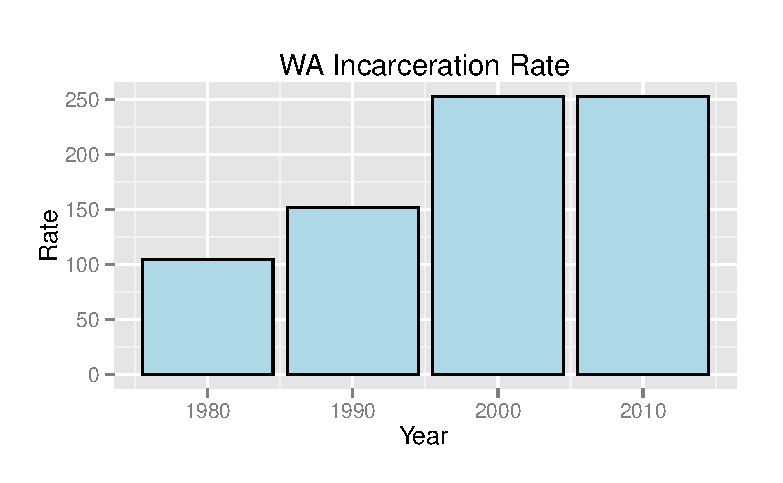
\includegraphics[scale = 0.9]{figures/wa_rate_over_time.eps}
    \caption{WA rate over time}
  \end{figure}

  \section{World Incarceration Rates}
  \begin{figure}[H]
    \centering
    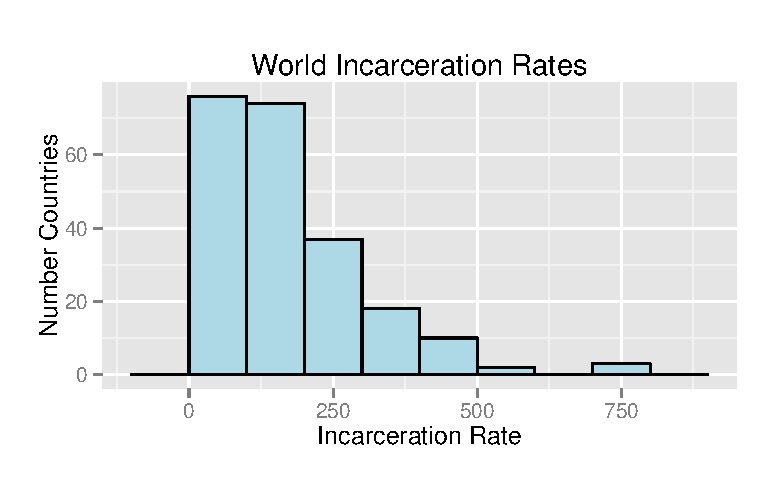
\includegraphics[scale = 0.9]{figures/wold_histogram.eps}
    \caption{World incarceration rate histogram}
  \end{figure}

  \begin{figure}[H]
    \centering
    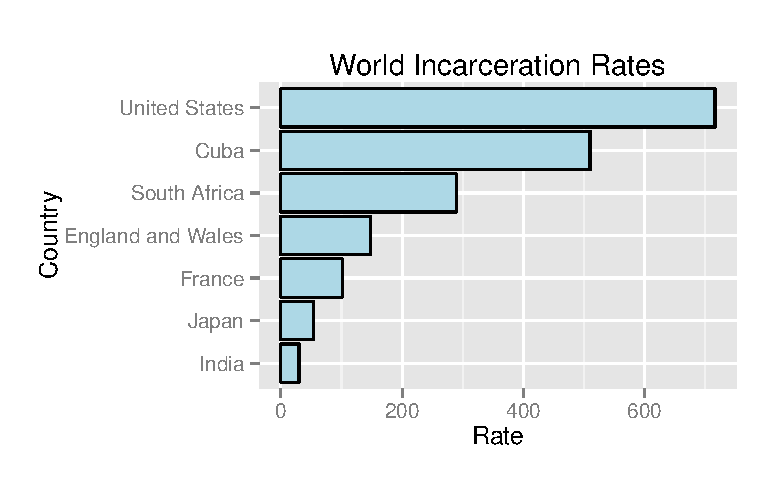
\includegraphics[scale = 0.9]{figures/sample_world_rates.eps}
    \caption{Sample countries}
  \end{figure}

\end{document}

